\documentclass{article}
\usepackage{multicol}
\usepackage{booktabs} 
\usepackage{blindtext}
\usepackage{float}  


\renewcommand{\refname}{Referencias}
\renewcommand{\tablename}{Tabla}

\title{Ejemplo de Documento Sweave}
\author{Carlos Schmidt}
\date{2024-07-22}

\usepackage{Sweave}
\begin{document}
\Sconcordance{concordance:Ejemplo.tex:Ejemplo.Rnw:1 12 1 1 0 15 1 1 8 1 5 6 1 1 30 19 %
1 1 35 1 2 6 1 1 27 18 1 1 36 1 2 6 1 1 27 17 1 1 45 1 2 38 1}


\maketitle

\textbf{Preguntas a las que este informe da respuesta:}
\begin{enumerate}
    \item ¿Cómo varían las tres motivaciones contempladas (extrínseca, intrínseca y prosocial) en función del sexo de los sujetos?
    \item ¿Cómo varían las tres motivaciones contempladas (extrínseca, intrínseca y prosocial) en función de la edad de los sujetos?
    \item ¿Cómo varían las tres motivaciones contempladas (extrínseca, intrínseca y prosocial) en función del nivel educativo de los sujetos?
    \item ¿Cuál es la distribución de los niveles de las tres motivaciones contempladas (extrínseca, intrínseca y prosocial) en los países de Europa occidental?
    \item ¿Cuál es la motivación principal de entre las tres contempladas (extrínseca, intrínseca y prosocial) en los países de Europa occidental?
\end{enumerate}





\section{Pregunta 1: ¿Cómo varían las tres motivaciones contempladas (extrínseca, intrínseca y prosocial) en función del sexo de los sujetos?
}

En esta sección, realizaremos un t-test para comparar las medias de la motivación intrínseca, extrínseca y prosocial por género.


Los resultados del t-test indican que hay diferencias estadísticamente significativas entre las medias de hombres y mujeres en las tres motivaciones contempladas. En concreto: las medias de las mujeres en motivación extrínseca (3.78) y motivación intrínseca (3.19) son más altas que las de los hombres (3.56 y 3.02), y la de los hombres lo es en motivación prosocial (2.01 frente a 1.85).

\begin{table}[h!]
\centering
\caption{Resultados del t-test para cada motivación por género}
\begin{tabular}{lccc}
  \toprule
  \textbf{Motivación} & \textbf{Media Hombres} & \textbf{Media Mujeres} & \textbf{p-valor} \\
  \midrule
  Motivación Prosocial & 2.01 & 1.85 & 0 \\
  Motivación Extrínseca & 3.56 & 3.78 & 0 \\
  Motivación Intrínseca & 3.02 & 3.19 & 0 \\
  \bottomrule
\end{tabular}
\end{table}

































Ejemplo de código de R ejecutable en fragmento de texto
La base de datos \texttt{df_filtered} tiene \emph{25827} observaciones.


\begin{multicols}{2}
[
\section{Texto con formato}
Algún texto aleatorio
]
\noindent \underline{Cursiva}\\  \emph{\blindtext}   \\   \underline{Typewritter}  \\   \texttt{\blindtext}
\end{multicols}


\begin{multicols}{2}
[
\subsection{Tamaño de fuente}
Modificando tamaño de fuente con palabras reservadas en \LaTex
]
{\Huge \blindtext}   {\scriptsize \blindtext}
\end{multicols}


\section{Tablas en LaTex}
\subsection{Tablas generadas desde Latex}
\begin{table}[h!]
\caption{Esto es un ejemplo de una tabla simple en Latex.}
\begin{tabular}{1 | c c}
\hline
\bf{Observación} & \bf{Var1} & \bf{Var2} \\
\hline
Individuo 1 & a & b \\
Individuo 2 & c & d \\
Individuo 3 & e & f \\
Individuo 4 & g & h \\
\hline
\end{tabular}
\end{table}



\subsection{Tablas generadas desde R}
\begin{table}[h!]
\centering
\caption{Resumen del Modelo}
\begin{tabular}{@{}lrrrr@{}}
\toprule
Variable & Estimate & Std. Error & t value & Pr(>|t|) \\
\midrule
(Intercept) &  1.6571639 & 0.25594569 &  6.474670 & 1.400102e-09 \\
Sepal.Length &  0.3777734 & 0.06556897 &  5.761466 & 4.867516e-08 \\
Petal.Length & -0.1875666 & 0.08349289 & -2.246498 & 2.619373e-02 \\
Petal.Width &  0.6257105 & 0.12337631 &  5.071561 & 1.195649e-06 \\
Speciesversicolor & -1.1602853 & 0.19329450 & -6.002681 & 1.503304e-08 \\
Speciesvirginica & -1.3982549 & 0.27714618 & -5.045189 & 1.344532e-06 \\
\bottomrule
\end{tabular}
\end{table}
begin{table}[h!]
centering
caption{Resumen del Modelo}
begin{tabular}{@{}lrrrr@{}}
toprule
Variable & Estimate & Std. Error & t value & Pr(>|t|) \
midrule
(Intercept) &  1.6571639 & 0.25594569 &  6.474670 & 1.400102e-09 \
Sepal.Length &  0.3777734 & 0.06556897 &  5.761466 & 4.867516e-08 \
Petal.Length & -0.1875666 & 0.08349289 & -2.246498 & 2.619373e-02 \
Petal.Width &  0.6257105 & 0.12337631 &  5.071561 & 1.195649e-06 \
Speciesversicolor & -1.1602853 & 0.19329450 & -6.002681 & 1.503304e-08 \
Speciesvirginica & -1.3982549 & 0.27714618 & -5.045189 & 1.344532e-06 \
bottomrule
end{tabular}
end{table}




\begin{Schunk}
\begin{Sinput}
> # Para establecer globalmente tamaño de gráficos
> knitr::opts_chunk$set(echo = FALSE, fig.height = 10, fig.width = 10)
\end{Sinput}
\end{Schunk}


\section{Gráficos en \LaTeX}
\subsection{Gráfico de motivaciones por sexo}

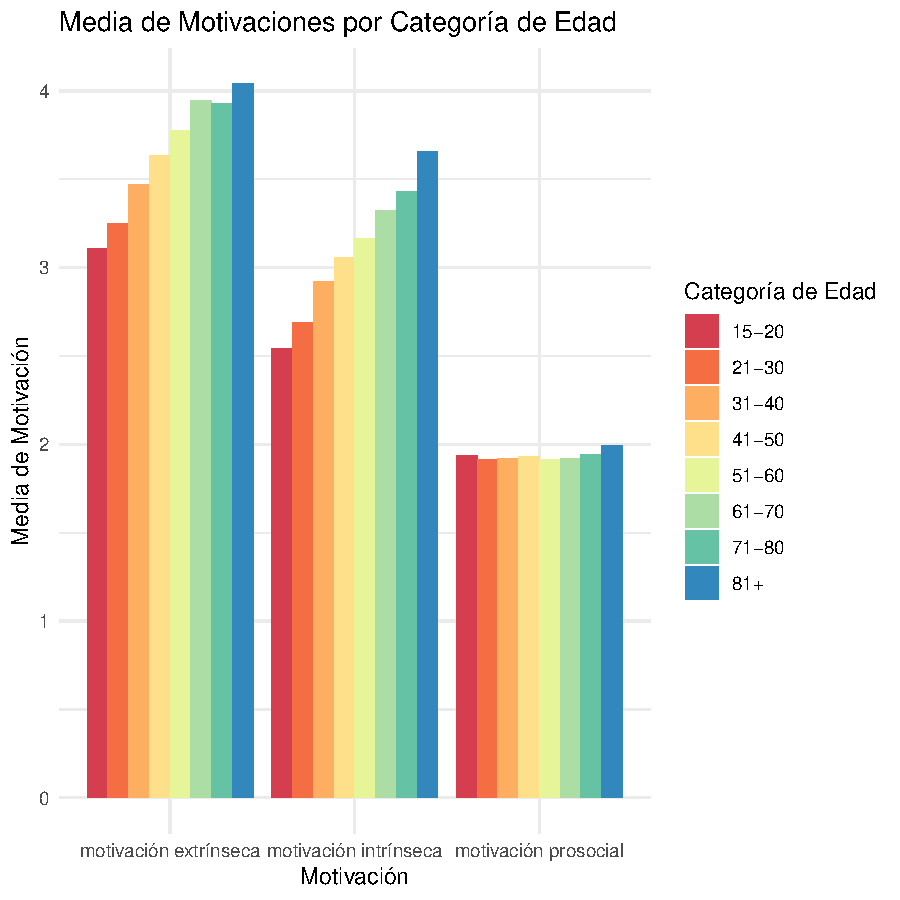
\includegraphics{Ejemplo-006}


\subsection{Gráfico de motivaciones por edad}
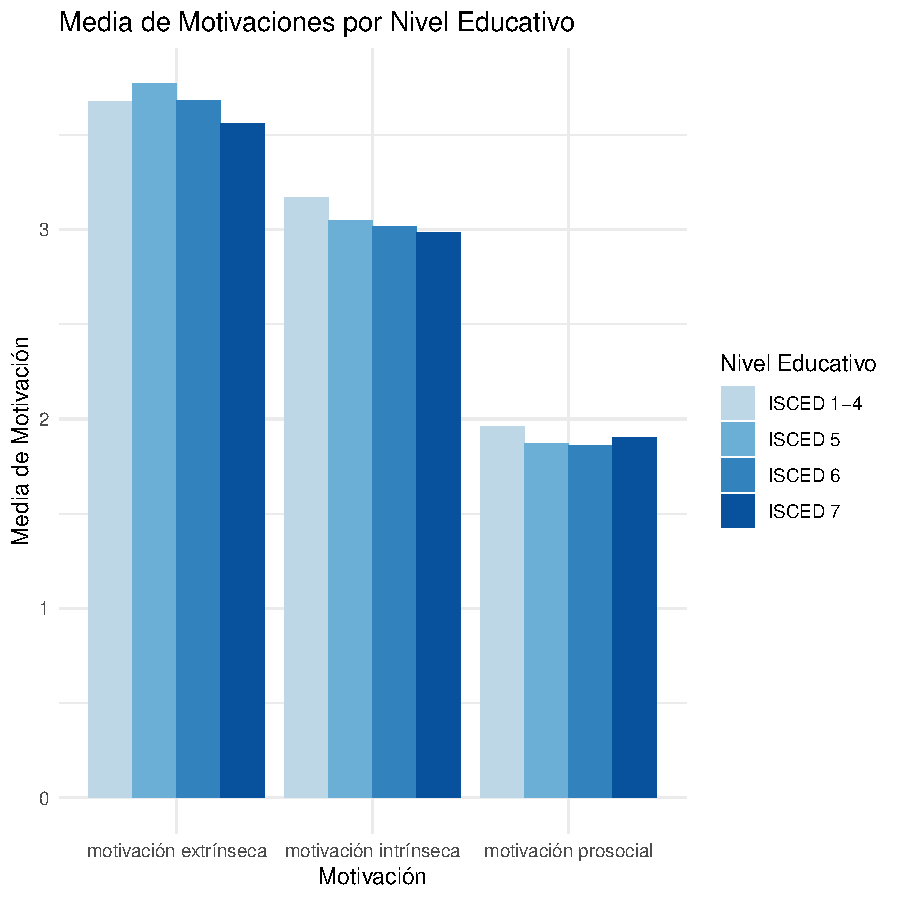
\includegraphics{Ejemplo-007}


\subsection{Gráfico de motivaciones por nivel educativo}
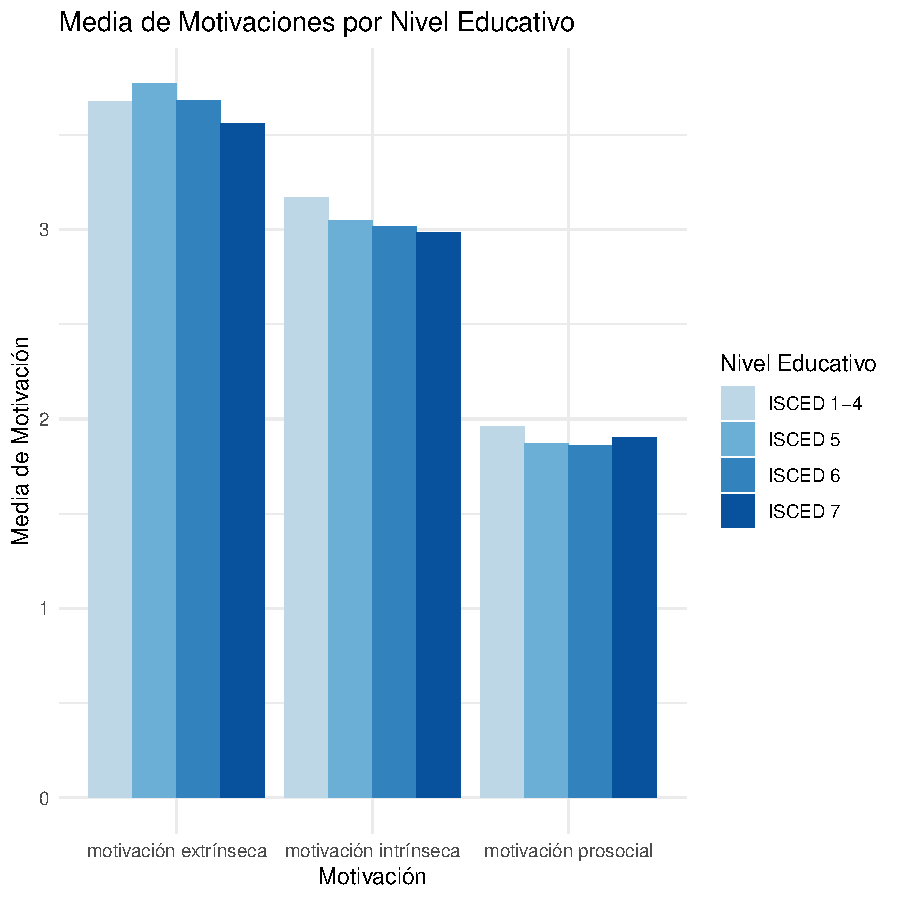
\includegraphics{Ejemplo-008}


\begin{table}

\caption{Media de las motivaciones por país}
\centering
\begin{tabular}[t]{lrrr}
\toprule
cntry & mean\_motprosoc & mean\_motextr & mean\_motintr\\
\midrule
AT & 1.83 & 3.30 & 3.02\\
BE & 1.93 & 3.42 & 2.94\\
CH & 1.78 & 3.52 & 2.72\\
DE & 1.82 & 3.76 & 3.04\\
DK & 1.80 & 3.67 & 2.78\\
\addlinespace
ES & 1.78 & 3.81 & 3.10\\
FI & 1.81 & 4.08 & 3.15\\
FR & 2.03 & 4.23 & 3.05\\
GB & 1.93 & 3.76 & 3.28\\
IE & 1.93 & 3.66 & 3.24\\
\addlinespace
IT & 2.17 & 3.09 & 3.54\\
NL & 2.02 & 3.56 & 3.04\\
NO & 2.05 & 3.89 & 3.16\\
PT & 2.08 & 3.75 & 3.17\\
SE & 1.98 & 4.04 & 3.08\\
\bottomrule
\end{tabular}
\end{table}








\end{document}

\begin{Schunk}
\begin{Sinput}
> 
\end{Sinput}
\end{Schunk}

